\

\vfill

\begin{center}
    \begin{quotation}
    \centering
    \textit{The more complex a system is, the more difficult its correctness verification will be.}\footnote{ \textsf{All notes are derived from oral presentations and written papers.}}
\end{quotation}
\end{center}
\vfill

\chapter{Introduction to Cybersecurity}


\section{Risk Estimation and Management}
\cite{01_introduction}
Complexity is an enemy of security, in fact, consequence of a succsseful attack are as follows:
\begin{itemize}
    \item Financial loss 
    \item Recovery cost
    \item Productivity loss 
    \item Business disruption
    \item Reputation damage
\end{itemize}

\begin{figure}[H]
    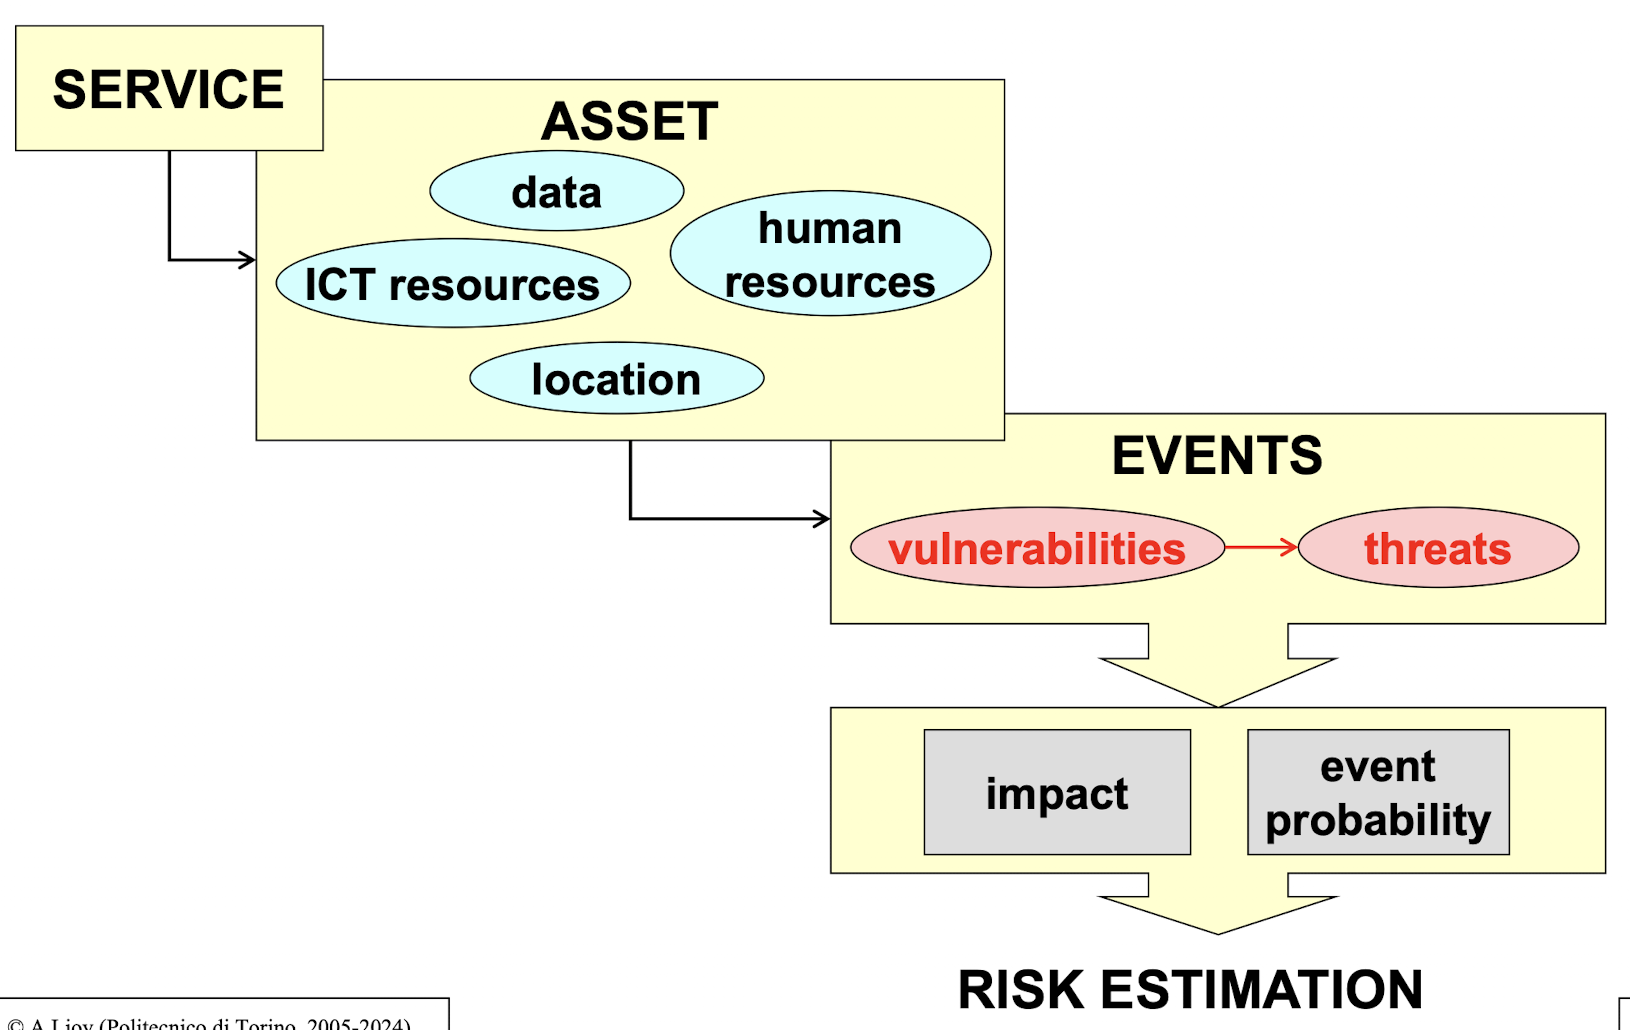
\includegraphics[width=\linewidth]{Images/Introduction/riskEvaluation.png}
    \caption{The risk estimation process}
\end{figure}

Terminolgy:
\begin{itemize}
    \item Asset: the set of goods, data and people needed for an IT service.
    \item Vulnerability: intrinsic weakness of an asset.
    \item Threat: possible deliberate action/accidental event that can produce the loss of a security property by exploiting a vulnerability.
    \item Attack: threat occurrence (deliberate action)
    \item (Negative) event: threat occurrence (accidental event)
\end{itemize}

Managing threats requires us to \textbf{prioritize risks}, considering not only the impact but also the available \textbf{time and budget}\footnote{A risk assessment matrix (or risk heat map) can be useful in this process}.

\begin{figure}[H]
    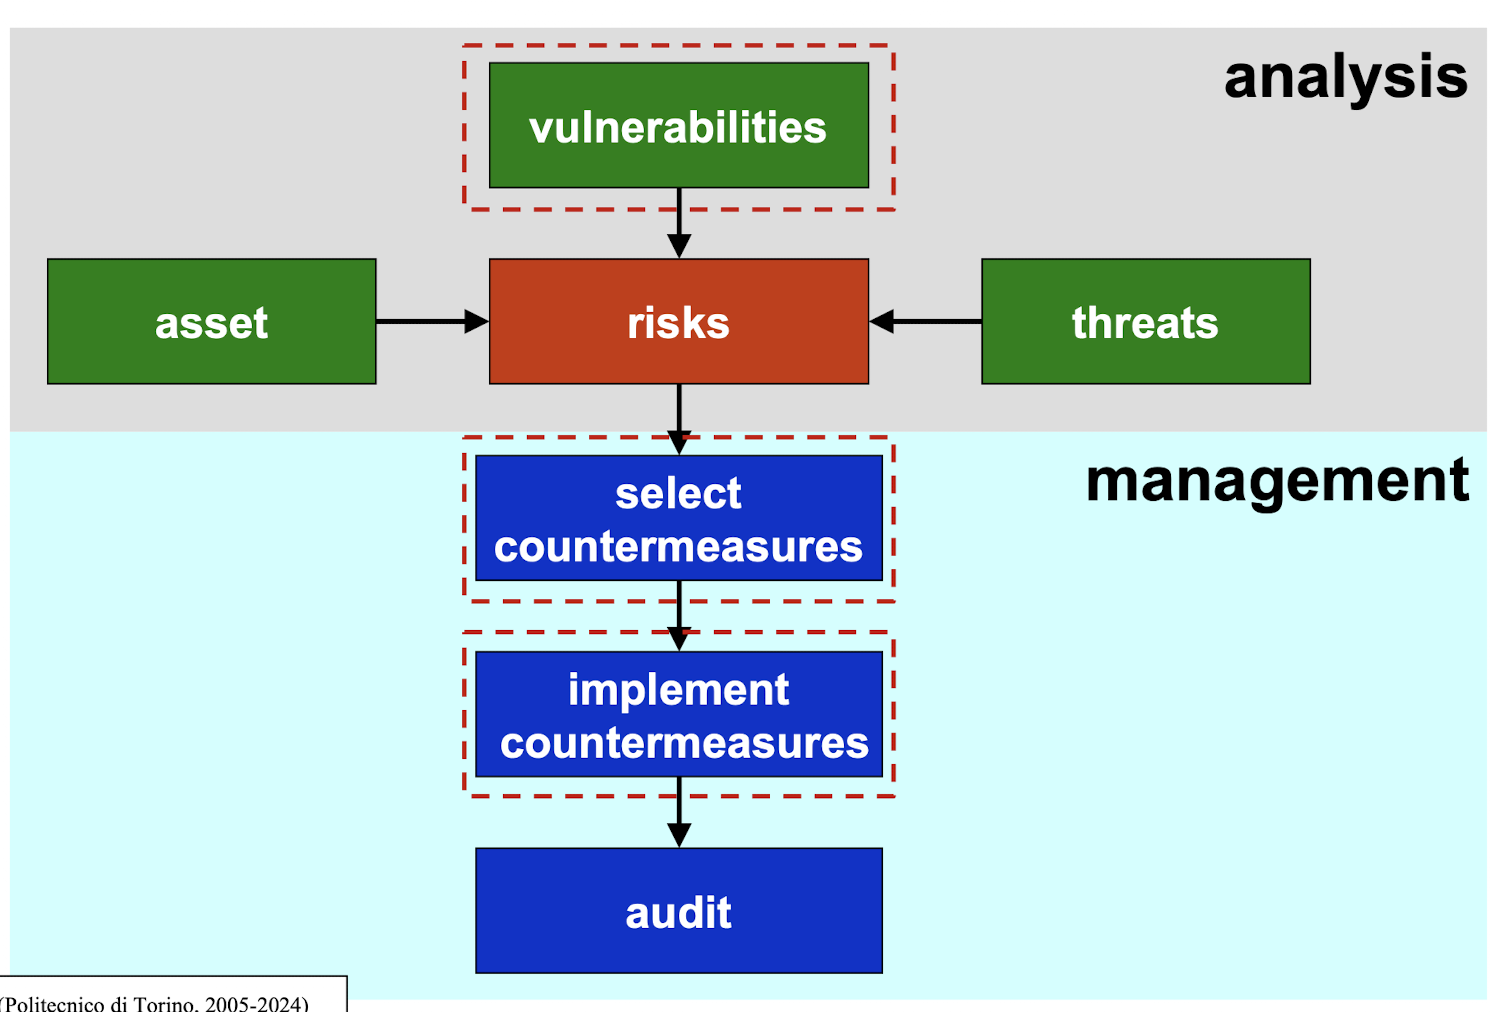
\includegraphics[width=\linewidth]{Images/Introduction/analysisAndManagement.png}
    \caption{Analysis and management of security}
\end{figure}